\documentclass[11pt,a4paper]{article}
\usepackage[utf8]{inputenc}
\usepackage[spanish]{babel}
\usepackage{amsmath}
\usepackage{amsfonts}
\usepackage{amssymb}
\usepackage{graphicx}
\usepackage[left=2cm,right=2cm,top=2cm,bottom=2cm]{geometry}
\title{Universidad Politécnica de la Zona Metropolitana de Guadalajara}
\begin{document}

\maketitle


\begin{figure}[h]
\begin{center}

\includegraphics[scale=1]{1.jpeg}
\end{center}
\end{figure}

\begin{center}
\section{Giro de un motor}
\end{center}

\begin{center}
\author{Sistemas Electrónicos de Interfaz\\
Barrera Vazquez Omar\\
Ing. Mecatrónica 4B}
\end{center}

\newpage

\section{Un motor y sus componentes}

Los motores de CD se componente básicamente por dos partes un \emph{rotor} y un \emph{estátor} los cuales hacen posible el giro circular  con eje fijo de un motor, hay mas tipos de variaciones en cuanto motores, especialmente tres tipos \emph{unipolares, bipolares y multifase}. 

\subsection{Estátor}

Es la parte metálica conformada por un bloque de laminas encimadas que acumularan las bobinas (\emph{normalmente de cobre}) o bobina, el cual le dará la determinación de motor unipolar, bipolar o multifase.


\subsection{Rotor}

El rotor es la parte que se encuentra en el centro, un eje metálico imantado que cruza de un extremo a otro al motor, este responderá  a la polaridad de las bobinas del motor según sus componentes, podemos apreciar las partes en la \emph{figura 1:}

\begin{figure}[h]
\begin{center}
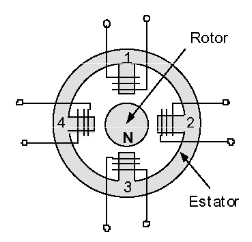
\includegraphics[scale=0.5]{2.png}
\caption{Ubicación de rotor y estátor}
\end{center}
\end{figure}

\section{Motor unifase}

El motor unifase es un claro ejemplo de un motor a pasos, el cual trabaja con un eje central de imán permanente varias bobinas en el estátor. Las bobinas en el estátor son las que le dan la dirección del giro al motor, al ser polarizadas por una corriente el rotor se ve atraído en la dirección polarizada. Para que el rotor pueda girar en distintos puntos y direcciones, es necesario que vaya por secciones, no puede brincarse la polarización y atracción de una bobina, por consecuente tiene que hacer el recorrido de manera secuencial, un ejemplo en la \emph{figura 2:}

\begin{figure}[h]
\begin{center}
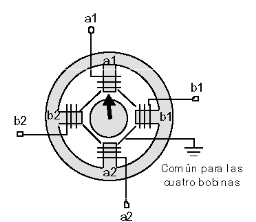
\includegraphics[scale=0.6]{3.png}
\caption{secuencia de giro del motor}
\end{center}
\end{figure}

\newpage

\subsection{Giro secuencial de motor unifase}
Como se observo en la \emph{figura 2} un motor de 4 fases que es convocado para un giro de 180 grados en el cual tiene que transistor por una fase para llegar a su bobina de destino. Hay tablas que nos ayudan a ver la manera secuencial del cambio de posición de un motor como lo muestra la siguiente \emph{tabla 1:}


\begin{center}
\begin{tabular}{|c|c|c|c|c|}
\hline 
Estado & a1 & a2 & a3 & a4 \\ 
\hline 
0 & 1 & 0 & 0 & 0 \\ 
\hline 
1 & 0 & 1 & 0 & 0 \\ 
\hline 
2 & 0 & 0 & 1 & 0\\ 
\hline 
3 & 0 & 0 & 0 & 0\\
\hline
\end{tabular} 
\end{center}

Entre mas fases \emph{(bobinas)} haya en un motor, mas combinaciones podremos encontrar para el avance. Una de las posibilidades que se pueden encontrar en un motor de este tipo es el una ubicación centrada entre dos fases, esto activando dos bobinas que estén de manera continua quedando una ubicación como lo muestra la \emph{figura 3:}

\begin{figure}[h]
\begin{center}
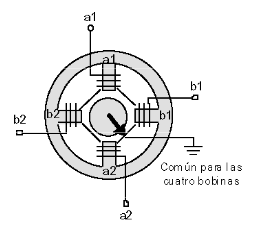
\includegraphics[scale=0.6]{4.png}
\end{center}
\end{figure}

Esto permite controlar la ubicación del rotor del motor de una manera precisa, pero otro problema es cuando se habla de motores de CD que giran a gran velocidad, si se requiere controlar la dirección del giro del motor, \emph{¿que factores incluirían para hacerlo posible?}, observe la sección 4:

\section{Puente H}

El puente H es un circuito simple que por medio de interruptores modifica el flujo de la corriente y esta a su vez la dirección del giro del motor de CD. Su funcionamiento básico es la combinación de 4 interruptores, estos pueden ser \emph{relevadores} o para un control mas automático los \emph{MOSFET} encapsulados parecidos al  transistor  pero con capacidades de alta potencia en la electrónica.

Un diagrama básico representado para un puente H es la \emph{figura 5} que se compone por relevadores o interruptores:

\begin{figure}[h]
\begin{center}
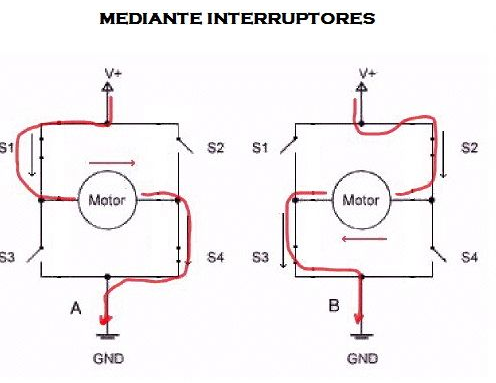
\includegraphics[scale=0.3]{5.png}
\caption{diseño básico de puente H}
\end{center}
\end{figure}

\newpage

\subsection{Puente H con MOSFET}

El puente H con MOSFET trabaja de manera igual que un \emph{puente H} con interruptores, solo que de una manera de control automatizada. Funciona al igual que un transistor, solo que con una capacidad de potencia mas alta al igual que temperaturas elevadas, mantiene 3 pines denominados \emph{gate, drain y source}. Por lo que el voltaje de alimentación no pasara del source al drain sin recibir un voltaje de pulso en el gate, estos pulsos pueden ser controlados desde un procesador según los requerimientos del circuito, se puede observar un \emph{puente H con MOSFET} en la \emph{figura 6:} \cite{ainversores}

\begin{figure}[h]
\begin{center}
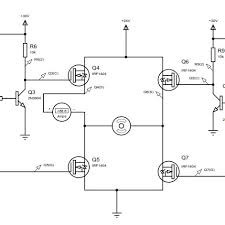
\includegraphics[scale=0.8]{6.png}
\end{center}
\end{figure}


\section{síntesis del giro de un motor}

Entre los aspectos a repasar de este documento son los siguientes:

\begin{itemize}

\item El control de presicion del movimiento de un motor puede estar dado por sus fases
\item Su velocidad estará dada por los voltajes y corrientes en su rotor y estátor
\item La dirección del giro de un motor se puede controlar por un circuito básico denominado \emph{puente H}
\item Para un control de la dirección del giro se pueden usar interruptores, relevadores y MOSFET. 


\bibliographystyle{apalike} 
\bibliography{ref.bib}




\end{itemize}



\end{document}